\section{量化}

\begin{quotation}
本节讨论如何通过量化将命题函项转变为命题。我们将介绍全称量词和存在量词的概念及符号表示,分析它们之间的逻辑关系,并探讨如何使用量化符号来表达不同类型的普遍命题,从而为理解更复杂的逻辑结构奠定基础。
\end{quotation}

\subsection{从命题函项到命题}

用个体常元代人个体变元,并不是从命题函项获得命题的唯一方式。通过概括或量化程序也可以得到命题。谓项通常不仅仅出现在单称命题中。例如,命题"每个事物是有死的"和"有些事物是漂亮的"含有谓项,但不是单称命题,因为它们不含有任何特定个体的名称。相反,作为普遍命题,它们不特别指称任何特定个体。

第一个命题可以用各种不同的逻辑等价的方式表示:或者表示为"所有事物都是有死的",或者表示为:

给定不管任何个体事物,它都是有死的。

在后一种表述中,语词"它"是一个关系代词,回指该陈述中前面的语词 "事物"。用字母 $x$ ,即个体变元,代替代词"它"及其先行词,我们可以把第一个普遍命题重写为:

给定任何 $x, x$ 是有死的。

或者,用前一节所介绍的符号,我们可以写成:

给定任何 $x, M x$ 。

尽管命题函项 $M x$ 不是一个命题,但我们这里有了一个含有它的表述式,而这个表述式是命题。短语"给定任何 $x$"习惯上用符号"$(x)$"表示,称为全称量词。上述第一个普遍命题可以完全符号化为:\\
(x)$M x$

\subsection{存在量化与全称量化}

第二个普遍命题,即"有些事物是漂亮的",也可以表达成:

至少存在这样一个事物,它是漂亮的。

在后一个表述中,语词"它"也是一个关系代词,回指语词"事物"。用个体变元 $x$ 代替代词"它"及其先行词,我们可以把第二个普遍命题重写为:

至少存在这样一个 $x, x$ 是漂亮的。

或者,我们可以用给定符号把它写成:

至少存在这样一个 $x, B x$ 。

同样,尽管 $B x$ 是一个命题函项而不是命题,但我们这里又有一个含有它的表述式,这个表述式是命题。短语"至少存在这样一个 $x$"习惯上用符号"$(\exists x)$"表示,称为存在量词。第二个普遍命题可以完全符号化为:\\
$(\exists x) B x$

于是我们看到,命题可以用列举方法从命题函项生成,即通过用个体常元代入个体变元,或者可以用概括方法生成,即在它的前面放一个全称词或存在量词。

现在请考虑:一个命题函项的全称量化式 $(x) M x$ 为真,当且仅当,它的所有代人例都为真;这正是普遍性的意义之所在。很显然,一个命题函项的存在量化式 $(\exists x) M x$ 为真,当且仅当,它至少有一个真代人例。我们假定(没人会否认这一点)至少存在一个个体。在这种非常弱的假定

下,每个命题函项必定至少有一个代人例,这个实例或真或不真。但可以确定的是,在这种假定下,如果一个命题函项的全称量化式为真,那么它的存在量化式也必定为真。也就是说,如果每个 $x$ 都是 $M$ ,那么,如果至少存在一个事物,则这个事物是 $M$ 。

\subsection{否定与量化}

到此时为止,只举了单称肯定命题作为命题函项的代人例。 $M x(x$ 是有死的)是一个命题函项。 $M s$ 是它的一个实例,是一个单称肯定命题,即"苏格拉底是有死的"。但并非所有命题都是肯定的。一个人可以否认苏格拉底是有死的,即 $\sim M s$ ,"苏格拉底不是有死的"。如果 $M s$ 是 $M x$ 的一个代入例,那么,~Ms可以看成是命题函项 $\sim M x$ 的一个代人例。因此,我们可以超出前一节所介绍的简单谓述,把我们的命题函项概念扩大到能包括否定符"~"。

如下所示,使用否定符可以丰富我们对量化的理解。从下述普遍命题出发:

没有任何事物是完美的。

我们可以把它解释为:

每个事物都是不完美的。

它又可以写成:

给定不管任何个体事物,它不是完美的。

它可以改写成:

给定任何 $x, x$ 不是完美的。

如果用 $P$ 符号化属性"是完美的",用刚才给出的符号(量词和否定符),我们可以把这个命题("没有任何事物是完美的")表示为 $(x) \sim P x$ 。

\subsection{量词间的逻辑关系}

现在我们可以列出并举例说明全称量化和存在量化之间的一系列重要关系。

第一,(全称)普遍命题"每个事物都是有死的",被(存在)普遍命题"有些事物不是有死的"否定。我们可以用符号说成,( $x$ )$M x$ 被 ( $\exists x$ )~$M x$ 否定。因为它们每个都是另一个的否定,我们当然可以说 (从有否定符的那个开始),下述双条件陈述是必然真的、逻辑真的:

$$
\sim(x) M x \stackrel{\stackrel{\mathrm{~T}}{=}(\exists x) \sim M x}{ }
$$

第二,"每个事物都是有死的"正好表示了"不存在任何不是有死的事物"所表示的东西——这可以表述成另一个逻辑真的双条件陈述:

$$
(x) M x \stackrel{\mathrm{T}}{=} \sim(\exists x) \sim M x_{0}
$$

第三,很清楚,(全称)普遍命题"没有任何事物是有死的",被(存在)普遍命题"有些事物是有死的"否定。用符号我们可以说 $(x) \sim M x$被( $x$ )$M x$ 否定。既然它们每个都是另一个的否定,我们当然可以说(还从有否定符的那个开始),下列双条件陈述是必然的、逻辑真的:

$$
\sim(x) \sim M x \stackrel{\stackrel{\mathrm{~T}}{=}}{(\exists x) M x}
$$

第四,"每个事物都不是有死的"正好表示了"不存在任何有死的事物"所表示的东西——这可以表述成另一个逻辑真的双条件陈述:

$$
(x) \sim M x \stackrel{\mathrm{T}}{=} \sim(\exists x) M x
$$

这四个逻辑真的双条件陈述阐明了全称量词和存在量词的相互关系。任何一个否定符在量词之前的命题,(利用这些逻辑真的双条件陈述)我们都可以用另一个与其逻辑等价但量词前面没有否定符的命题替换之。现在以符号 $\phi$(希腊字母 phi)替换例示谓词 $M$(有死的),$\phi$ 代表任何一个简单谓词,我们立即可列出下面这四个双条件陈述式:

$$
\begin{aligned}
& {\left[(x) \phi_{x}\right] \stackrel{\mathrm{T}}{=}\left[\sim(\exists x) \sim \phi_{x}\right]} \\
& {\left[(\exists x) \phi_{x}\right] \stackrel{\mathrm{T}}{=}\left[\sim(x) \sim \phi_{x}\right]} \\
& {\left[(x) \sim \phi_{x}\right] \stackrel{\mathrm{T}}{=}\left[\sim(\exists x) \phi_{x}\right]} \\
& {\left[\exists(x) \sim \phi_{x}\right] \stackrel{\mathrm{T}}{=}\left[\sim(x) \phi_{x}\right]}
\end{aligned}
$$

\subsection{量词逻辑方阵}

全称量化和存在量化之间的一般关系,可以用图 10-1 中的方阵进行

更图示化的描述。\\
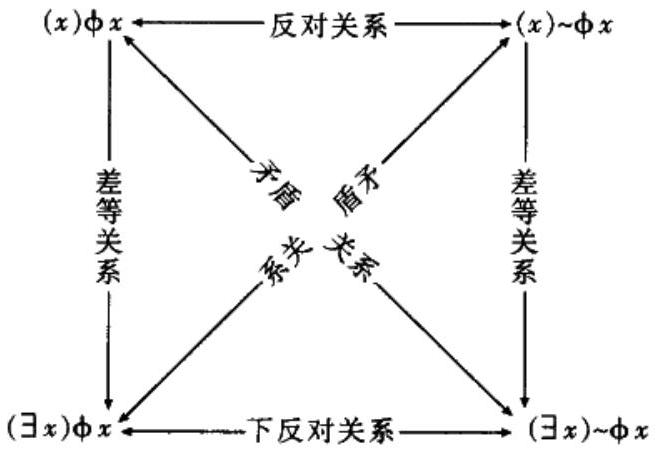
\includegraphics[width=\textwidth]{images/2025_05_15_6a28331d5e7c993ad07ag-463.jpg}

图10—1\\
继续假定至少存在一个个体,就该方阵我们可以说:\\
1.顶端的两个命题是反对关系;就是说,它们可以同时为假,但不能同时为真。

2.底端的两个命题是下反对关系;就是说,它们可以同时为真,但不能同时为假。

3.对角线相反两端的命题是矛盾关系;它们中一个为真,则另一个必定为假。

4.在方阵的每侧,下面命题的真被它正上方命题的真所蕴涵。 

\begin{center}
\fbox{\parbox{0.95\textwidth}{
\textbf{本节要点}
\begin{itemize}
\item \textbf{量化的基本概念}:
  \begin{itemize}
  \item 量化是将命题函项转变为命题的方法
  \item 区别于列举法(通过代入个体常元)
  \item 通过量词可表达普遍命题
  \end{itemize}
\item \textbf{两种基本量词}:
  \begin{itemize}
  \item 全称量词(x):表示"对所有x都成立"
  \item 存在量词(∃x):表示"至少存在一个x使...成立"
  \item 全称量化为真当且仅当所有代入例为真
  \item 存在量化为真当且仅当至少有一个代入例为真
  \end{itemize}
\item \textbf{量词与否定的关系}:
  \begin{itemize}
  \item ~(x)φx 等价于 (∃x)~φx
  \item (x)φx 等价于 ~(∃x)~φx
  \item ~(x)~φx 等价于 (∃x)φx
  \item (x)~φx 等价于 ~(∃x)φx
  \end{itemize}
\item \textbf{量词逻辑方阵}:
  \begin{itemize}
  \item 描述全称肯定、全称否定、特称肯定、特称否定命题间的关系
  \item 包含反对关系、下反对关系和矛盾关系
  \item 展示量化命题间的逻辑蕴涵关系
  \end{itemize}
\end{itemize}
}}
\end{center} 